\subsection{Mask R-CNN}
\begin{frame}{}
    \LARGE Instance Segmentation: \textbf{Mask R-CNN}
\end{frame}

\begin{frame}[allowframebreaks]{Mask R-CNN}
    \textbf{Mask R-CNN Overview}
    \begin{itemize}
        \item \textbf{Developed on top of Faster R-CNN}
        \item Faster R-CNN outputs:
        \begin{itemize}
            \item Class label
            \item Bounding-box offset
        \end{itemize}
        \item Mask R-CNN adds a third branch:
        \begin{itemize}
            \item Predicts object mask for each candidate
        \end{itemize}
        \item Performs \textbf{Instance Segmentation} (per-object masks; extensible to keypoint/pose estimation)
    \end{itemize}

\framebreak

    \begin{figure}
    \centering
    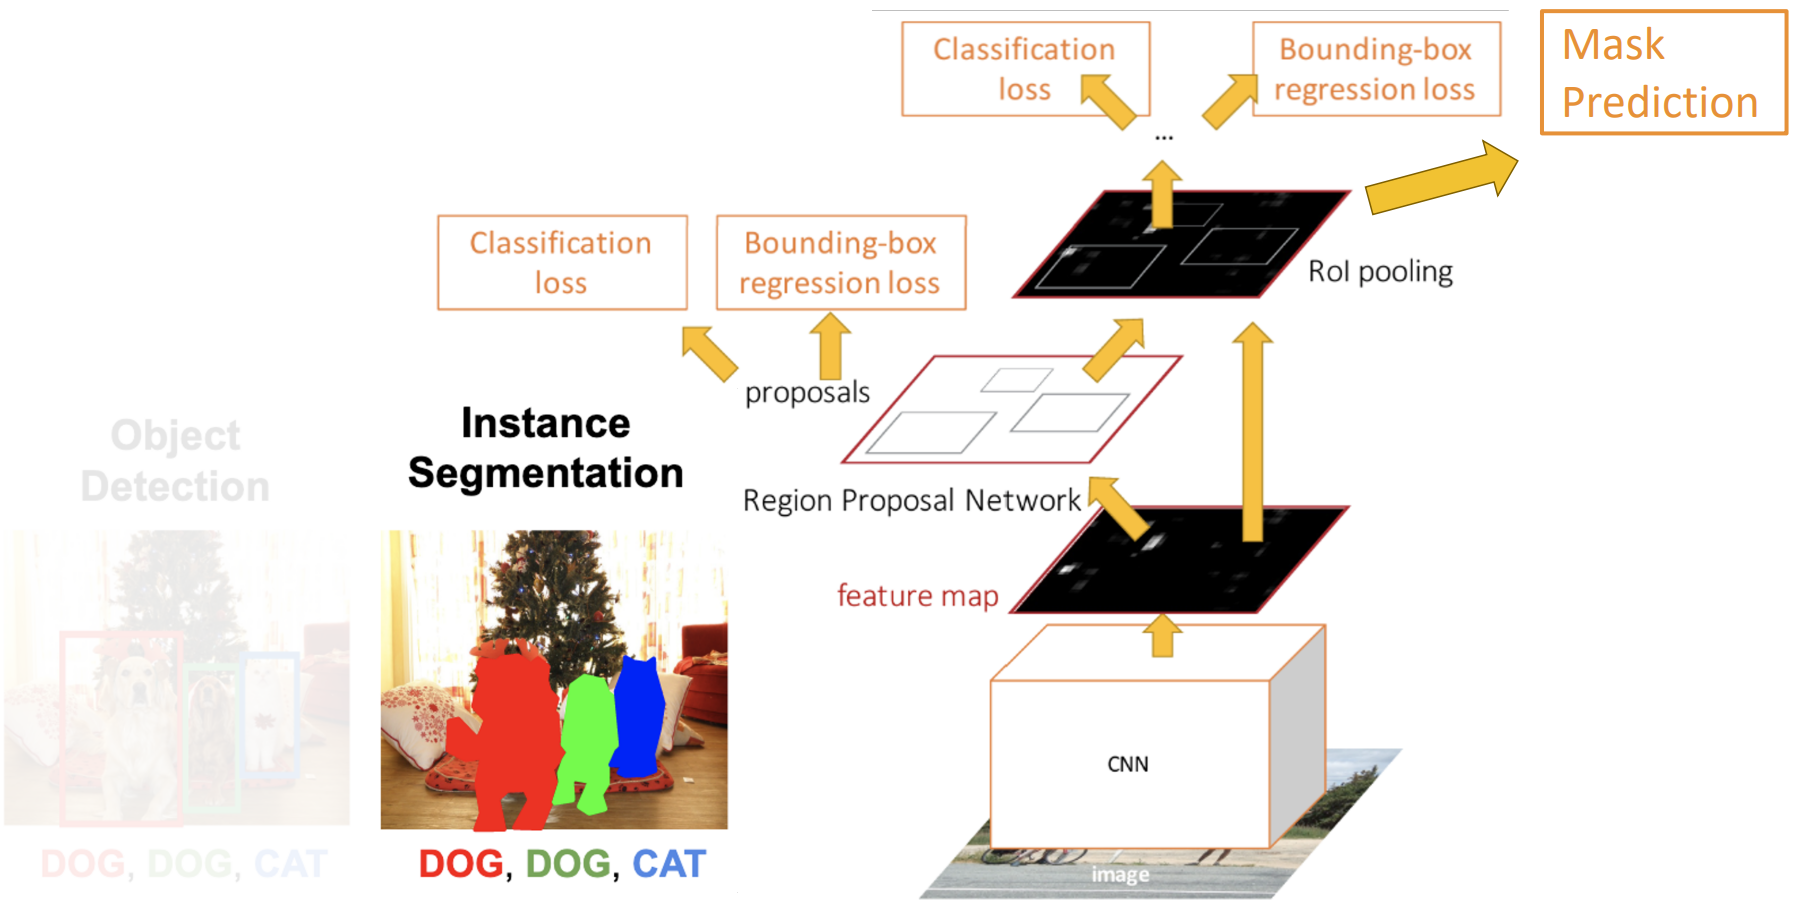
\includegraphics[width=1.0\textwidth,height=0.85\textheight,keepaspectratio]{images/object-detect/ins_6.png}
    \caption*{\scriptsize He et al., “Mask R-CNN”, ICCV 2017.}
    \end{figure}

\framebreak

    \begin{figure}
    \centering
    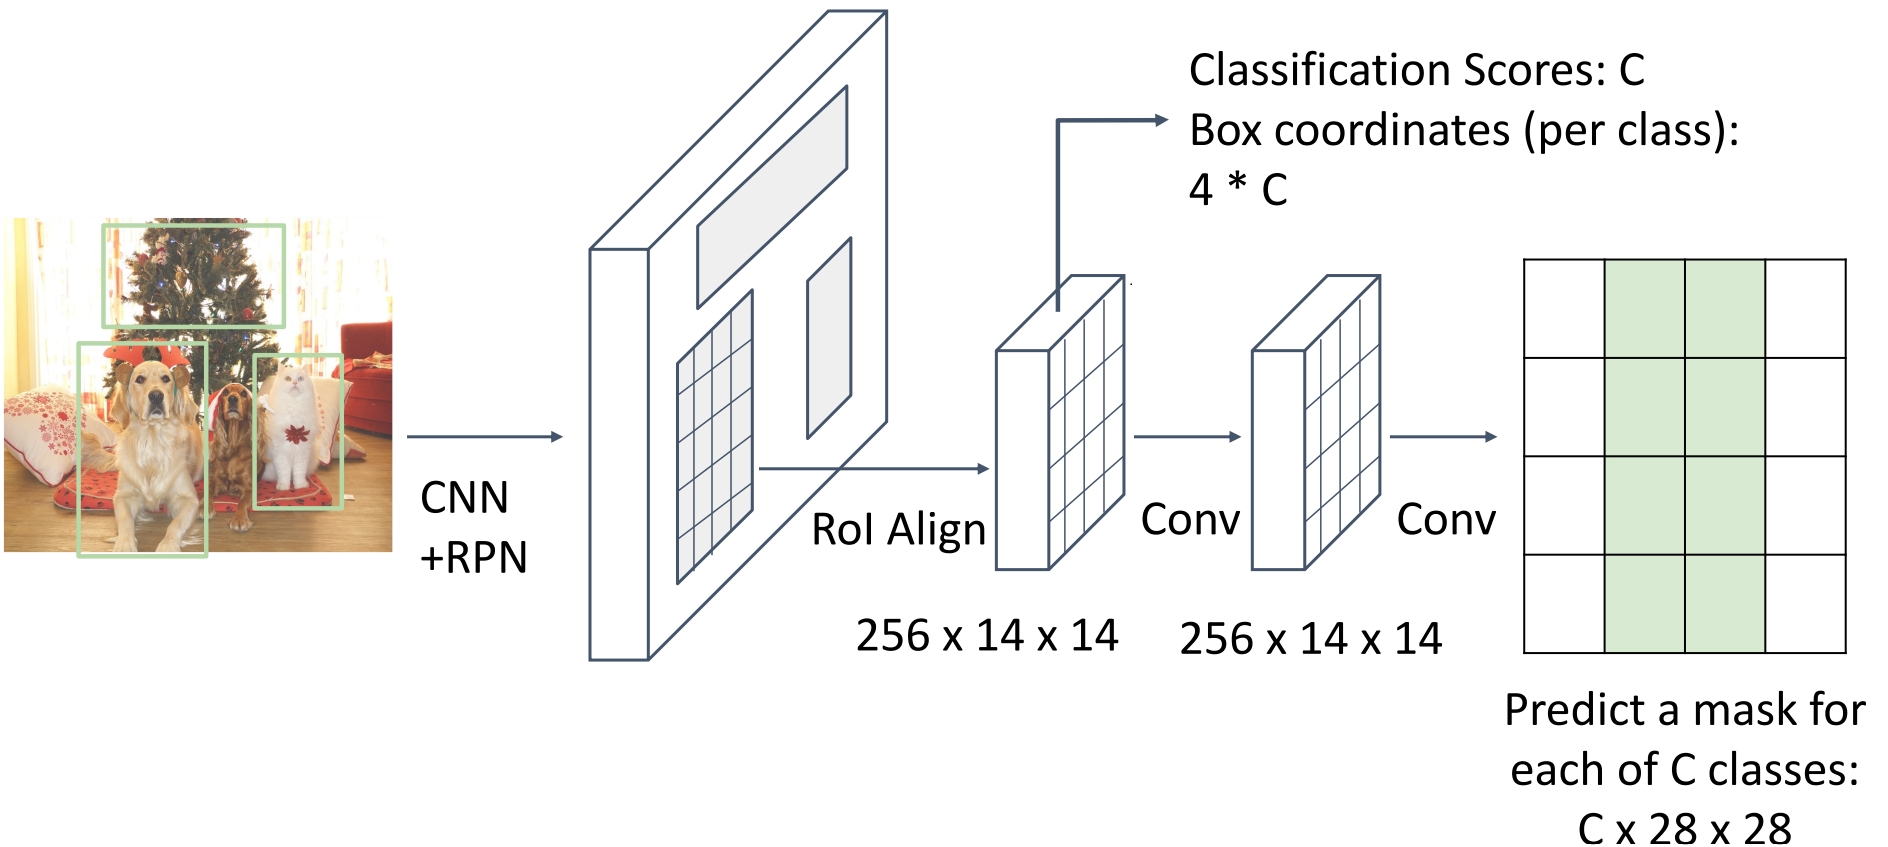
\includegraphics[width=1.0\textwidth,height=0.85\textheight,keepaspectratio]{images/object-detect/ins_7.png}
    \caption*{\tiny Source: UMich EECS 498 (2022), Lecture 15: Image Segmentation, slide 79 (figure from He et al., ``Mask R-CNN'', ICCV 2017)}
    \end{figure}

\framebreak

    \textbf{Advantages of Mask R-CNN}
    \begin{itemize}
        \item \textbf{Simplicity}: Simple to train
        \item \textbf{Performance}: Outperforms previous methods, at 5 fps (195\,ms per image on a Tesla M40)
        \item \textbf{Efficiency}: Very efficient, small overhead compared to Faster R-CNN
        \item \textbf{Flexibility}: Can perform detection and estimation tasks simultaneously
    \end{itemize}
\end{frame}

\begin{frame}{Mask R-CNN: Example Training Targets}
    \begin{figure}
        \centering
        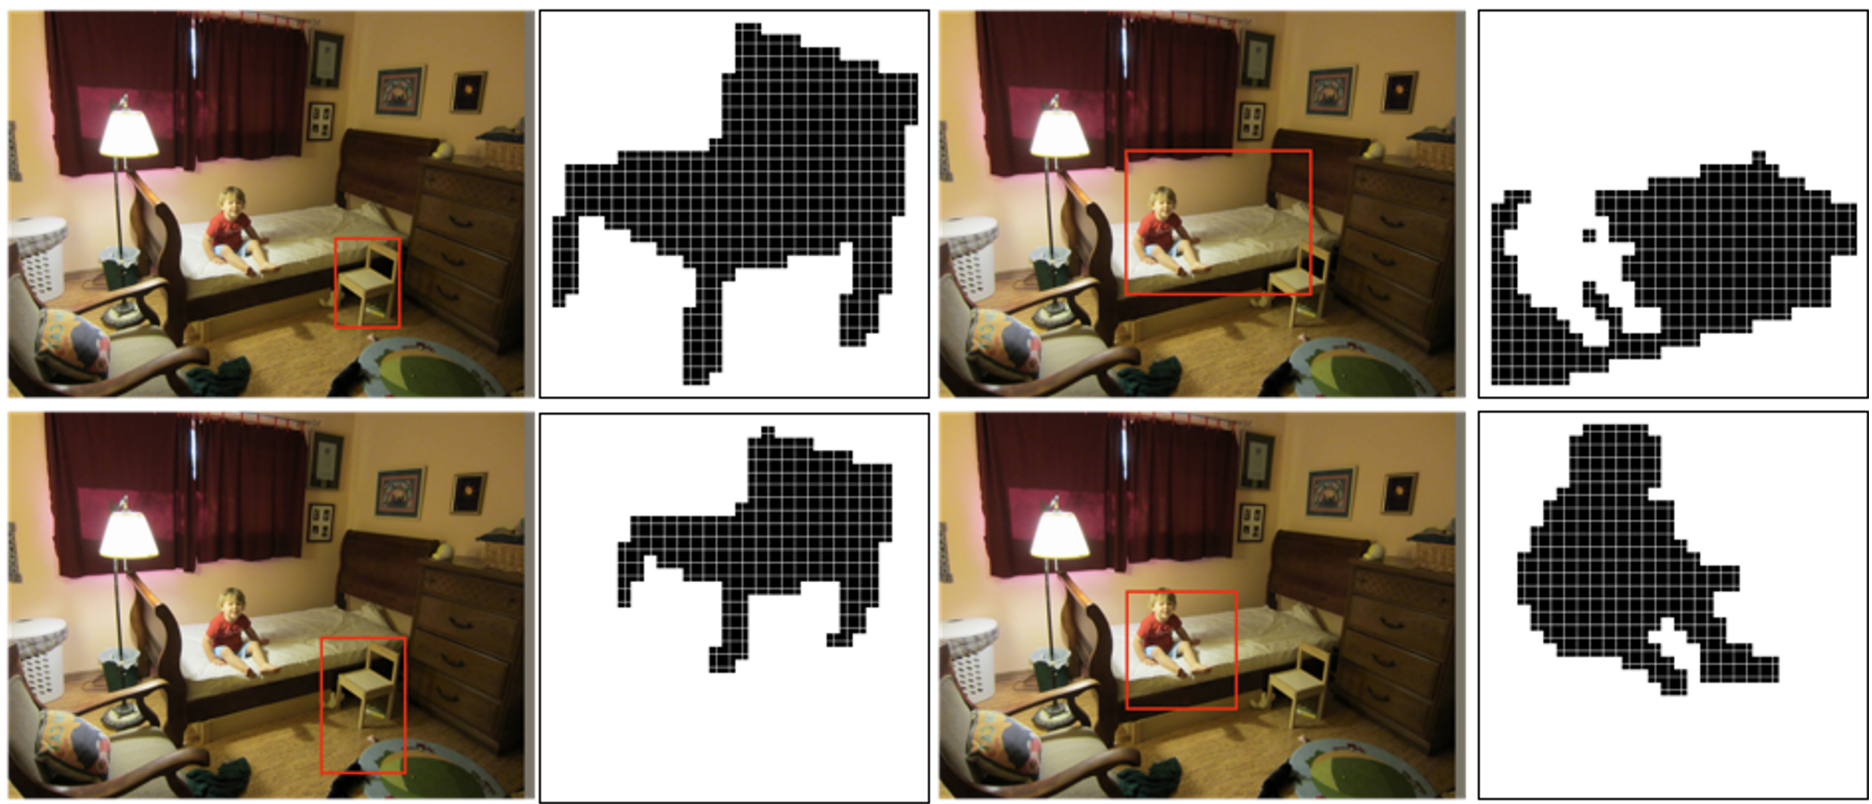
\includegraphics[width=1.0\textwidth,height=1.0\textheight,keepaspectratio]{images/object-detect/ins_8.png}
        \caption*{\tiny Source: UMich EECS 498 (2022), Lecture 15: Image Segmentation, slide 83 (figure from He et al., ``Mask R-CNN'', ICCV 2017)}
    \end{figure}
\end{frame}

\begin{frame}{Mask R-CNN: Very Good Results!}
    \begin{figure}
        \centering
        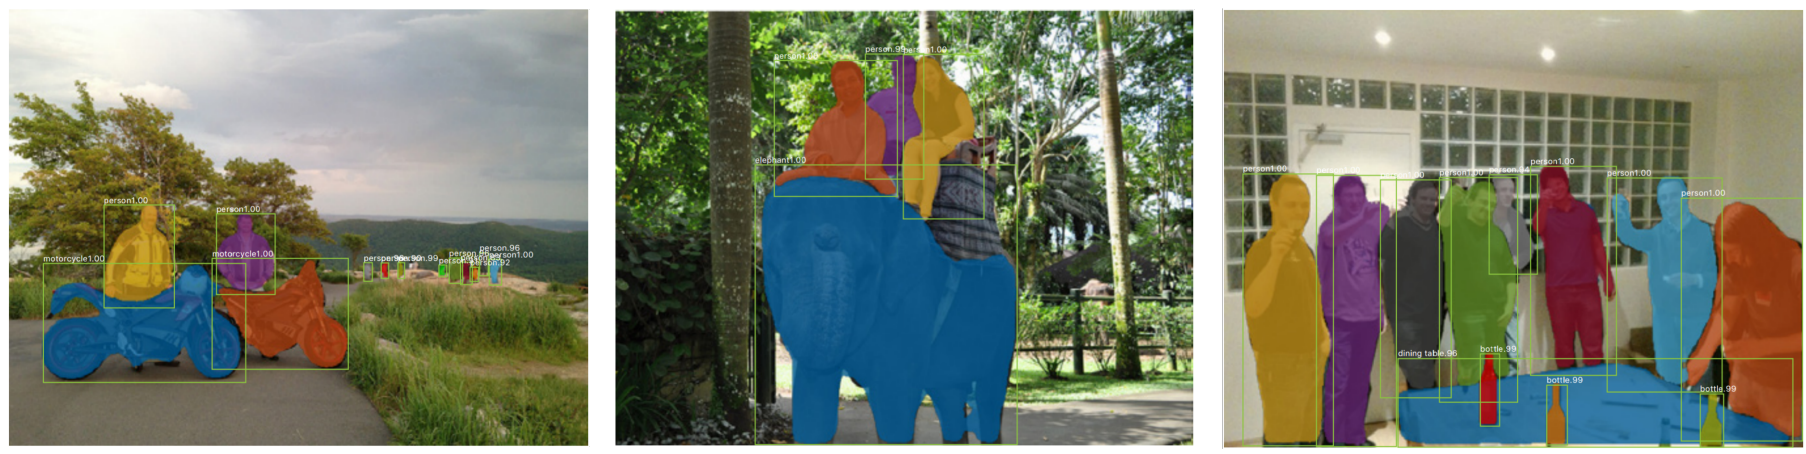
\includegraphics[width=1.0\textwidth,height=1.0\textheight,keepaspectratio]{images/object-detect/ins_9.png}
        \caption*{\tiny Source: UMich EECS 498 (2022), Lecture 15: Image Segmentation, slide 84 (figure from He et al., ``Mask R-CNN'', ICCV 2017)}
    \end{figure}
\end{frame}